% This file was created with tikzplotlib v0.10.1.
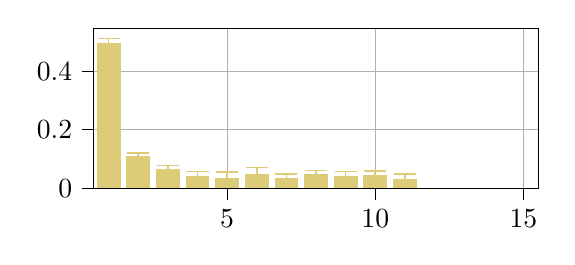
\begin{tikzpicture}

\definecolor{burlywood221204119}{RGB}{221,204,119}
\definecolor{darkgray176}{RGB}{176,176,176}

\begin{axis}[
height=1.4222438079424382in,
tick align=outside,
tick pos=left,
width=2.8444876158848764in,
x grid style={darkgray176},
xmajorgrids,
xmin=0.5, xmax=15.5,
xtick style={color=black},
y grid style={darkgray176},
ymajorgrids,
ymin=0, ymax=0.547440194428687,
ytick style={color=black}
]
\draw[draw=none,fill=burlywood221204119] (axis cs:0.6,0) rectangle (axis cs:1.4,0.497440194428687);
\draw[draw=none,fill=burlywood221204119] (axis cs:1.6,0) rectangle (axis cs:2.4,0.110117588239728);
\draw[draw=none,fill=burlywood221204119] (axis cs:2.6,0) rectangle (axis cs:3.4,0.0665906527163901);
\draw[draw=none,fill=burlywood221204119] (axis cs:3.6,0) rectangle (axis cs:4.4,0.0408899603690654);
\draw[draw=none,fill=burlywood221204119] (axis cs:4.6,0) rectangle (axis cs:5.4,0.0341011262069239);
\draw[draw=none,fill=burlywood221204119] (axis cs:5.6,0) rectangle (axis cs:6.4,0.0497727163998173);
\draw[draw=none,fill=burlywood221204119] (axis cs:6.6,0) rectangle (axis cs:7.4,0.0359048158767614);
\draw[draw=none,fill=burlywood221204119] (axis cs:7.6,0) rectangle (axis cs:8.4,0.0478589847727953);
\draw[draw=none,fill=burlywood221204119] (axis cs:8.6,0) rectangle (axis cs:9.4,0.0412724978246361);
\draw[draw=none,fill=burlywood221204119] (axis cs:9.6,0) rectangle (axis cs:10.4,0.0437072987870088);
\draw[draw=none,fill=burlywood221204119] (axis cs:10.6,0) rectangle (axis cs:11.4,0.0323441643781863);
\path [draw=burlywood221204119, semithick]
(axis cs:1,0.48271739918586)
--(axis cs:1,0.512162989671514);

\path [draw=burlywood221204119, semithick]
(axis cs:2,0.098920178787996)
--(axis cs:2,0.121314997691461);

\path [draw=burlywood221204119, semithick]
(axis cs:3,0.0561313572372929)
--(axis cs:3,0.0770499481954874);

\path [draw=burlywood221204119, semithick]
(axis cs:4,0.0250891884214061)
--(axis cs:4,0.0566907323167247);

\path [draw=burlywood221204119, semithick]
(axis cs:5,0.0129927045118768)
--(axis cs:5,0.0552095479019711);

\path [draw=burlywood221204119, semithick]
(axis cs:6,0.0292828566900165)
--(axis cs:6,0.0702625761096181);

\path [draw=burlywood221204119, semithick]
(axis cs:7,0.0236928568412065)
--(axis cs:7,0.0481167749123164);

\path [draw=burlywood221204119, semithick]
(axis cs:8,0.0357774534938624)
--(axis cs:8,0.0599405160517283);

\path [draw=burlywood221204119, semithick]
(axis cs:9,0.0251207908469161)
--(axis cs:9,0.0574242048023561);

\path [draw=burlywood221204119, semithick]
(axis cs:10,0.0278238187882365)
--(axis cs:10,0.059590778785781);

\path [draw=burlywood221204119, semithick]
(axis cs:11,0.0168846573193419)
--(axis cs:11,0.0478036714370308);

\addplot [semithick, burlywood221204119, mark=-, mark size=4, mark options={solid}, only marks]
table {%
1 0.48271739918586
2 0.098920178787996
3 0.0561313572372929
4 0.0250891884214061
5 0.0129927045118768
6 0.0292828566900165
7 0.0236928568412065
8 0.0357774534938624
9 0.0251207908469161
10 0.0278238187882365
11 0.0168846573193419
};
\addplot [semithick, burlywood221204119, mark=-, mark size=4, mark options={solid}, only marks]
table {%
1 0.512162989671514
2 0.121314997691461
3 0.0770499481954874
4 0.0566907323167247
5 0.0552095479019711
6 0.0702625761096181
7 0.0481167749123164
8 0.0599405160517283
9 0.0574242048023561
10 0.059590778785781
11 0.0478036714370308
};
\end{axis}

\end{tikzpicture}
